\section{Durchführung des Versuches}
\label{sec:Durchführung}
\subsection{Versuchsaufbau}
Im Folgenden wird die zur Messung verwendete Versuchsapparatur, die in Abbildung \ref{fig:apparatur} dargestellt ist, erläutert.

\noindent
Die Lichtquelle ist durch eine Halogen-Lampe mit einem Emissionsspektrum, das überwiegend im Infrarotbereich liegt, realisiert. 
Zunächst wird das Licht durch eine Sammellinse parallelisiert und dann anschließend durch eine rotierende Sektorscheibe in 
einzelne Lichtimpulse zerteilt. 
Diese sogenannte Wechsellichtmethode hat den Vorteil, dass das Rauschen der Photowiderstände später in einem Selektivverstärker
herausgefiltert werden kann.

\noindent
Die einzelnen Lichtimpulse werden daraufhin in einem Glan-Thompson Prisma in zwei senkrecht 
zueinander polarisierte Teilstrahlen aufgespalten. Es folgt ein Elektromagent mit einer Öffnung, in welcher die Probe eingeführt
wird. Nachdem das Licht die Probe durchdrungen hat, wird mit einem Interferenzfilter eine ausgewählte Wellenlänge des Lichts 
selektiert, sodass dieses möglichst monochromatisch ist. Erneut wird der Lichtstrahl in einem Glan-Thompson Prisma in zwei 
senkrecht zueinander polarisierte Teile aufgespalten, die dann auf jeweils einen Photowiderstand gerichtet sind. Die Photowiderstände
übersetzen das optische Signal in eine elektrische Spannung. Die Spannungssignale beider Photowiderstände werden dann an einen
Differenzverstärker weitergeleitet. Wenn beide Strahlen den gleichen Betrag und die gleiche Phase besitzen, verschwindet die Spannung
im Differenzverstärker. Über den bereits erwähnten Selektivverstärker wird das Signal an ein Oszilloskop weiter gegeben, sodass
es abgelesen werden kann.   

\begin{figure}[H]
    \centering
    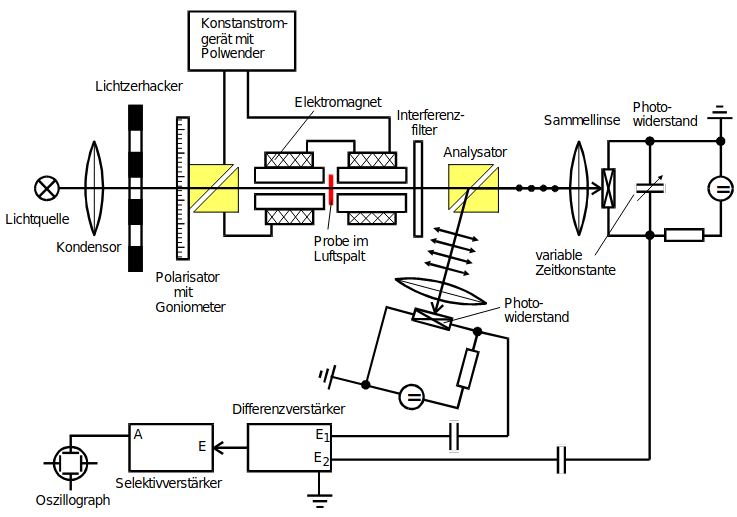
\includegraphics[scale=0.7]{pictures/Versuchsaufbau.png}
    \caption{Schematische Darstellung der Versuchsapparatur. \cite{Versuchsbeschreibung}}
    \label{fig:apparatur}
\end{figure}

\subsection{Justage}
Um bei der Messung sinnvolle Ergebnisse zu erhalten, muss die Anlage vor Inbetriebnahme justiert werden. 

\noindent
Eingangs werden die Probe und der Interferenzfilter aus der Apparatur entfernt, sodass die Funktionstüchtigkeit der
Polarisationsvorrichtung überprüft werden kann. Bei idealer Stellung des Prismas sollte die Lichtintensität in dem 
Austrittsfenster verschwinden. Zudem sollten die Strahlen mittig auf die Photowiderstände treffen. 
Die rotierende Sektroscheibe sowie der Selektivverstärker werden auf eine Frequenz von $\SI{450}{\hertz}$ geregelt. 
Der Gütefaktor wird auf den Wert $Q=\num{100}$ eingestellt. 
Nachdem die Probe und der Interferenzfilter wieder montiert wurden, wird der Polarisator so gedreht, dass die Spannung auf Null
abfällt. 

\subsection{Messprogramm}
Zu Beginn wird die Flussdichte des Magnetfeldes in Richtung des einfallenden Lichts unter Verwendung einer Hallsonde ausgemessen.
Diese Messung wird bei maximalem Feldstrom für verschiedene Weglängen vorgenommen.

\noindent
Danach wird die Faraday-Rotation der hochreinen GaAs-Probe bestimmt. Hierbei werden durch mehrfaches Wechseln des Interferenzfilters 
neun verschiedene Wellenlängen im nahinfraroten Bereich verwendet. Für jede Magnetfeld-Polung wird ein Nullabgleich vorgenommen 
und der zugehörige Winkel notiert. Somit werden für jeden Filter zwei Winkel aufgenommen. Genau das gleich Vorgehen wird auch bei 
zwei verschiedenen n-dotierten GaAs-Probe vorgenomen. 